\documentclass[12pt]{report}
\usepackage[spanish]{babel}
\usepackage[utf8]{inputenc}
\usepackage{graphicx}
\usepackage{verbatim}
\usepackage{listings}
\usepackage{float}
\renewcommand*\thesection{\arabic{section}}

\begin{document}
	
	\begin{center}
		\textbf{Análisis de Algoritmos, Sem: 2018-1, 3CV1, Práctica 1, 08-2017}
		\newline
	\end{center}
	
	\begin{center}
		\LARGE Práctica 1: Determinación experimental de
		la complejidad temporal de un algoritmo.\\
	\end{center}
	
	\begin{center}
		\textbf{Blancas Pérez Bryan Israel}\\
	\end{center}
	
	\begin{center}
		Escuela Superior de Cómputo.\\
		Instituto Politécnico Nacional, México\\
		orionmunecaycanica@gmail.com\\
	\end{center}
	
	
	\textbf{\large Resumen: }Realizar los algoritmos convenientes para resolver los problemas planteados, y analizar de manera experimental, el número de operaciones que realizan éstos, para poder graficar los resultados y determinar su complejidad computacional.\newline\\
	\textbf{\large Palabras Clave: }Complejidad computacional, complejidad del algoritmo, operaciones, tiempo de ejecución.\\
	
	\section{Introducción}
		Un algoritmo, es un conjunto de instrucciones bien definidas, ordenadas y finitas que permiten llevar a cabo una actividad. Los algoritmos nos ayudan a resolver problemas de todo tipo, de manera que no haya lugar a dudas en el procedimiento.[1]\\
		Analizar un algoritmo es de vital importancia, ya que de ese análisis se obtendrá que tan eficiente es; particularmente en nuestro campo las ciencias de la computación, se desea que el algoritmo use la menor cantidad de recursos del computador (tiempo y memoria).\\
		En esta práctica se desarrollarán algoritmos para resolver los problemas planteados y posteriormente, se analizarán de manera experimental, graficando el tiempo de ejecución dependiendo de la entrada dada.\newpage
	
	
	\section{Conceptos Básicos}
	\textbf{Notación $\theta$:}
	La notación $\theta$ se puede interpretar como el conjunto que acota a $f(n)$ por arriba y por abajo, $\theta$ es un ajuste asintótico para $f(n)$. Expresado matemáticamente sería:\newline \\
	$Sea \ g(n) \ una \ funcion, \ entonces\newline \\
	\theta(g(n))=\{f(n) \ | \ \exists \ C_{0},C_{1},n_{0}>0 \ tal que \ 0\leq C_{0}g(n)\leq f(n)  \leq C_{1}g(n) \ \forall \ n\geq n_{0}\}$\newline
	
	\textbf{Notación $O$:}
	La notación $O$ se puede interpretar como el conjunto que acota a $f(n)$ por arriba. Expresado matemáticamente sería:\newline \\
	$Sea \ g(n) \ una \ funcion, \ entonces\newline \\
	O(g(n))=\{f(n) \ | \ \exists \ C,n_{0}>0 \ tal que \ 0\leq f(n)  \leq Cg(n) \ \forall \ n\geq n_{0}\}$\newline
	
	\textbf{Notación $\Omega$:}
	La notación $\Omega$ se puede interpretar como el conjunto que acota a $f(n)$  por abajo . Expresado matemáticamente sería:\newline \\
	$Sea \ g(n) \ una \ funcion, \ entonces\newline \\
	\Omega(g(n))=\{f(n) \ | \ \exists \ C,n_{0}>0 \ tal que \ 0\leq Cg(n)\leq f(n) \ \forall \ n\geq n_{0}\}$\newline
	
	En esta práctica se desarrollarán dos algoritmos. El primero de ellos, es un algoritmo para hacer la suma binaria de dos arreglos y el segundo es el algoritmo de Euclides para encontrar el MCD de un par de números, los cuales son pares de la seria de Fibonacci.\newpage
	
	\section{Experimentación y Resultados}	
	\textbf{Ejercicio 1.}\\
	Desarrollar e implementar un algoritmo de $Suma$ que sume dos enteros en notación binaria guardados en dos arreglos unidimensionales A y B de tamaño $n$, considerando $k \ = \ log_{2}(n)$.\newline \\
	Código fuente del algoritmo de $Suma$:
	\lstset{language=C, breaklines=true, basicstyle=\footnotesize}
	\lstset{numbers=left, numberstyle=\tiny, stepnumber=1, numbersep=10pt}
	\begin{lstlisting}
int suma(int a[],int b[],int n){
	int c[n],cont=1,i,acarreo=0;	
	cont++;
	for(i=n-1;i>=0;i--,cont++){
		c[i]=a[i]+b[i]+acarreo;	cont++;
		if(c[i]==2){ 		cont++;
			c[i]=0;		cont++;
			acarreo=1;	cont++;
		}
		else if (c[i]==3){	cont++;
			c[i]=1;		cont++;
			acarreo=1;	cont++;
		}
		else{			cont++;
			acarreo=0;	cont++;
		}
	}
	return cont;
}
	\end{lstlisting}
	
	La función suma, recibe dos arreglos (A y B) y el tamaño de éstos (n). Luego mediante un $for$, va recorriendo los arreglos de derecha a izquierda, sumando los números correspondientes. Dentro del $for$ hay dos condiciones para controlar el acarreo que se pueda generar al momento de hacer la suma. Cada que se encuentra el resultado de la suma, se guarda en la correspondiente posición del arreglo C. El contador $cont$, como lo acordamos en clase, funge como el tiempo de ejecución.\newpage
	
	
	Programa en ejecución\\
	\begin{figure}[H]
		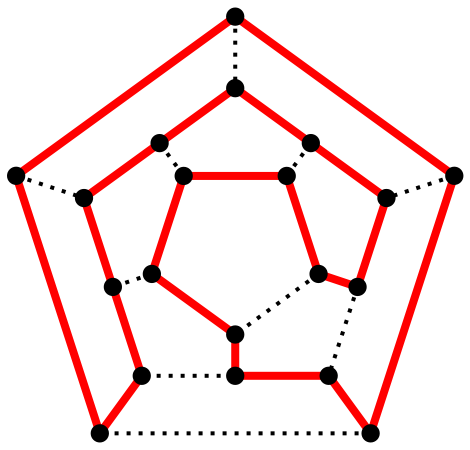
\includegraphics[width=4cm]{1.png}
		\centering
		\caption{Ejecución del programa 1.}
		\centering
	\end{figure}
	En la figura 1, se aprecia que el programa recibe como entrada el número, potencia de dos, que se interpretará como el tamaño de los arreglos. Como salida en la terminal, se muestra las sumas echas por el programa, empezando por los bit menos significativos de ambos arreglos.
	\begin{figure}[H]
		\includegraphics[height=6cm]{1_file.png}
		\centering
		\caption{output en archivo del programa 1.}
		\centering
	\end{figure}
	En la figura 2, se muestra la salida del programa 1 en el archivo. La primer columna representa el tamaño de los arreglos sumados y la segunda salida representa el tiempo de ejecución (cont) que se requirió para terminar exitosamente el programa.\newpage
	
	Gráfica de resultado.\\
		\begin{figure}[H]
			\includegraphics[width=14cm]{grafica1.png}
			\centering
			\caption{Gráfica del ejecicio 1.}
			\centering
		\end{figure}
	En la figura 3, se muestra la gráfica $T(n) vs n$, en la que los puntos marcados corresponden a los datos obtenidos en el archivo de la figura 2.
	La práctica pide proponer una función que acote por arriba a $T(n)$, en este caso la función propuesta es $y \ = \ 5x$, la cual se puede apreciar siempre por encima de $T(n)$ en la figura 3.\\
	
	Conclusiones del programa.\\
	Este es un algoritmo fácil de desarrollar, lo interesante desde mi punto de vista, fue ver el comportamiento que tiene dependiendo de la entrada, es decir, como se aprecia en la gráfica de la figura 3, este algoritmo es de orden lineal. \newpage
	
	\textbf{Ejercicio 2.}\\
	Implementar el algoritmo de $Euclides$ para encontrar el MCD de dos números enteros positivos m y n. En la ejecución existen dos modos, el primero es elegir dos números aleatorios entre 0 y 1000, y la segunda es encontrar el MCD de los números de la serie de Fibonacci.\newline \\
	Código fuente del algoritmo de $Euclides$:
	\lstset{language=C, breaklines=true, basicstyle=\footnotesize}
	\lstset{numbers=left, numberstyle=\tiny, stepnumber=1, numbersep=10pt}
	\begin{lstlisting}
int euclides(int m, int n){
	int r,cont=1;
	while (n!=0){
		cont++;
		r=m%n;	cont++;
		m=n;	cont++;	
		n=r;	cont++;
	}
	printf("mcd: %d\n",m); cont++;
	return cont;
}
	\end{lstlisting}
	
	La función euclides, recibe como parámetros dos números enteros positivos, a los cuales les calcula el MCD. EL contador (cont) utilizado funge como tiempo de ejecución. La función retorna el tiempo que se tardo en ejecutarse para que posteriormente ese dato pueda ser guardado en un archivo.\\
	
	
	Programa en ejecución\\
	\begin{figure}[H]
		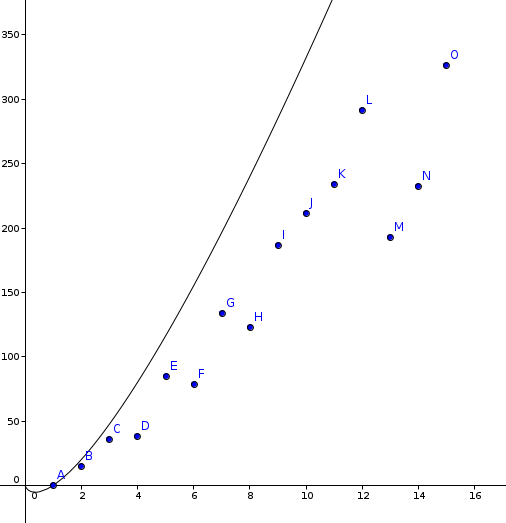
\includegraphics[height=5.5cm]{2.png}
		\centering
		\caption{Ejecución del programa 2.}
		\centering
	\end{figure}
	En la figura 4, se muestra que el programa recibe como entrada el número correspondiente a la elección del usuario. Como salida en la terminal, se muestra el MCD de los dos números analizados.
	\begin{figure}[H]
		\includegraphics[height=6cm]{2_file.png}
		\centering
		\caption{Output en archivo del programa 2.}
		\centering
	\end{figure}
	En la figura 4, se muestra la salida del programa 2 en el archivo. Las primeras dos columnas son los números a los que se les busco el MCD y la tercer columna representa el tiempo de ejecución (cont) que se requirió para calcular el MCD.\newpage
	
	Gráfica de resultado.\\
	\begin{figure}[H]
		\includegraphics[width=14cm]{1_2grafica.png}
		\centering
		\caption{Gráfica 1 del ejercicio 2.}
		\centering
	\end{figure}
	En la figura 6, se muestra la gráfica $T(n) vs n$, en la que los puntos marcados corresponden a los datos obtenidos en el archivo de la ejecución del programa 2 en modo random, tomando la coordenada sobre n (eje horizontal) como el número más grande de ambos.\\
	
	\begin{figure}[H]
		\includegraphics[width=14cm]{2_2grafica.png}
		\centering
		\caption{Gráfica 2 del ejercicio 2.}
		\centering
	\end{figure}
	En la figura 7, se muestra la gráfica $T(n) vs n$, en la que los puntos marcados corresponden a los datos obtenidos en el archivo de la figura 5, tomando la coordenada sobre n (eje horizontal) como el número más grande de ambos.\\
	La práctica pide proponer una función que acote por arriba a $T(n)$, en este caso la función propuesta es $y \ = \ 10log(x)$, la cual se puede apreciar siempre por encima de $T(n)$ en la figura 7.\newpage
		Conclusiones del programa.\\
	Es interesante notar del comportamiento de un algoritmo en el peor de los casos. En el caso del algoritmo de Euclides, el peor de los casos se presenta cuando se analizar los números de la serie de Fibonacci. En ese caso el algoritmo se comporta de manera logarítmica, sólo hace ver la gráfica para poder percatarse de ello. 
	
	\section{Conclusiones}
	Al momento de desarrollar los algoritmos no tenia ni idea del comportamiento que tendrían, pero al obtener los datos y graficarlos me di cuenta de que analizar un algoritmo nos brinda una forma de expresar el comportamiento de este mediante funciones matemáticas, y así, poder determinar cual algoritmo conviene más para la solución de un determinado problema. En lo general, no tuve problemas al desarrollar la práctica, ya que los problemas planteados eran fáciles de resolver. Al final los resultados fueron los esperados, una función lineal para el ejercicio 1 y una función logarítmica para el ejercicio 2, y eso me indica que los algoritmos fueron desarrollados e implementados de forma correcta.\\
		
	\section{Anexo}
	
	Resolver el siguiente problema.
	
	El siguiente algoritmo, es un algoritmo de ordenamiento llamado por selección (Select-Sort). Calcula el orden de complejidad en el peor de los casos.
	
	\lstset{language=C, breaklines=true, basicstyle=\footnotesize}
	\lstset{numbers=left, numberstyle=\tiny, stepnumber=1, numbersep=10pt}
	\begin{lstlisting}
Select-Sort(A[0,...,n-1])
  for j <- 0 to j <= n-2 do
    k <- j 
    for i <- j+1 to i <= n-1 do
      if A[i] < A[k] then
        k <- i
    intercambia(A[j],A[k])
	\end{lstlisting}
	\newpage
	\begin{table}[htbp]
		\begin{center}
			\begin{tabular}{|l|l|l|}
				\hline
				\multicolumn{3}{|c|}{Análisis del Algoritmo} \\ 
				\hline
				\textbf{Línea de Código} & \textbf{Tiempo Ejecución} & \textbf{Número de Ejecuciones}\\
				\hline
				2 & C1 & $n$ \\ \hline
				3 & C2 & $n-1$ \\ \hline
				4 & C3 & $\sum_{0}^{n-1}ti$ \\ \hline
				5 & C4 & $\sum_{0}^{n-1}(ti-1)$ \\ \hline
				6 & C5 & $\sum_{0}^{n-1}(ti-1)$ \\ \hline
				7 & C6 & $n-1$ \\ \hline
			\end{tabular}
			\caption{Análisis del algoritmo}
			\label{tabla:analisis}
		\end{center}
	\end{table}
Encontrando el orden de complejidad.\\
	
T(n) = C1n + C2(n-1) + C3 $\sum_{0}^{n-1}ti$ + C4 $\sum_{0}^{n-1}(ti-1)$ + C5 $\sum_{0}^{n-1}(ti-1)$ + C6(n-1).\\

Pero.\\

	\begin{table}[htbp]
		\begin{center}
			\begin{tabular}{|l|l|l|}
				\hline
				\multicolumn{3}{|c|}{Encontrando ti} \\ 
				\hline
				\textbf{j} & \textbf{i} & \textbf{ti}\\
				\hline
				0 & $1 \leq i \leq n-1$ & $n$ \\ \hline
				1 & $2 \leq i \leq n-1$ & $n-1$ \\ \hline
				2 & $3\leq i \leq n-1$ & $n-2$ \\ \hline
				... & ... & ... \\ \hline
				j & . & $n-j$ \\ \hline
			\end{tabular}
			\caption{Encontrando ti}
		\end{center}
	\end{table}

Encontrar.\\
	
T(n) = C1n + C2(n-1) + C3 $\sum_{0}^{n-1}(n-j)$ + C4 $\sum_{0}^{n-1}(n-j-1)$ + C5 $\sum_{0}^{n-1}(n-j-1)$ + C6(n-1).\\

T(n) = C1n + C2(n-1) + C3 $\sum_{0}^{n-1}(n)$- C3 $\sum_{0}^{n-1}(j)$ + C4 $\sum_{0}^{n-1}(n)$- C4 $\sum_{0}^{n-1}(j)$- C4 $\sum_{0}^{n-1}(1)$ + C5 $\sum_{0}^{n-1}(n)$- C5 $\sum_{0}^{n-1}(j)$-C5 $\sum_{0}^{n-1}(1)$ + C6(n-1).\\


T(n) = C1n + C2(n-1) + C3$(n^{2}-(n)(n+1)/(2))$ + (C4+C5) $(n^{2}-(n)(n+1)/2-n)$ + C6(n-1).\\

T(n) = C1n + C2(n-1) + C3$(n^{2}-(n^{2}+n)/(2))$ + (C4+C5) $(n^{2}-(n^{2}+n))/2-n)$ + C6(n-1).\\

Como se aprecia, el máximo exponente de n es 2, es decir, $n^{2}$. Por lo tanto la ecuación queda de la siguiente manera.\\

T(n)= A$n^{2}$+B$n$+C.\\

$ por \ lo \ tanto \ \ \ T(n) \ \epsilon \ \theta (n^{2})$

	\section{Bibliografía}
	
	[1] es.wikipedia,org/wiki/algoritmo
	
\end{document}